\documentclass[10pt]{standalone}

\usepackage{graphicx}
\usepackage{tikz}

\begin{document}
\begin{tikzpicture}



\draw[fill] (0,0) circle(.1)coordinate(A) node[below]{A};
\draw[very thick, -latex] (A)--++(110:1);


\draw[fill] (5,2) circle(.1)coordinate(B) node[below]{B};


\draw[fill=red!30] (2,3)rectangle(4,1)node[midway]{obstacle};



\draw[red, dashed] (A) to [out=110, in=180] (3,3.5) to[out=0, in=90](B);

\draw[blue, dashed] (A) -- (4.1,.9) -- (B);

\path (-.3,-2)node[above right]{
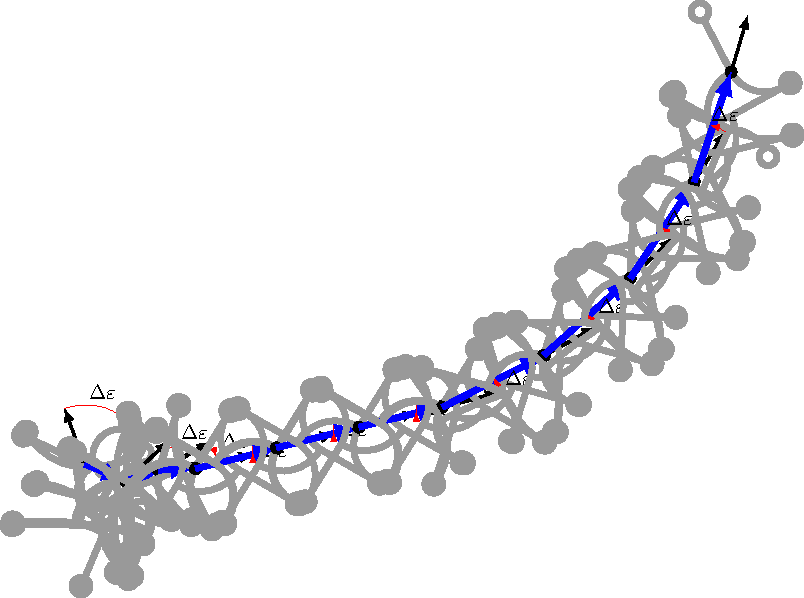
\includegraphics[scale=.4]{example.pdf}};

\path (6,5)node[below right, blue, align=left]{
	{[curve right supertight]} \\ 
	{[curve right]}*2 \\ 
	{[straight]}*4 \\ 
	{[curve left]}*4};

\path (-.7,-.3)node[above right]{
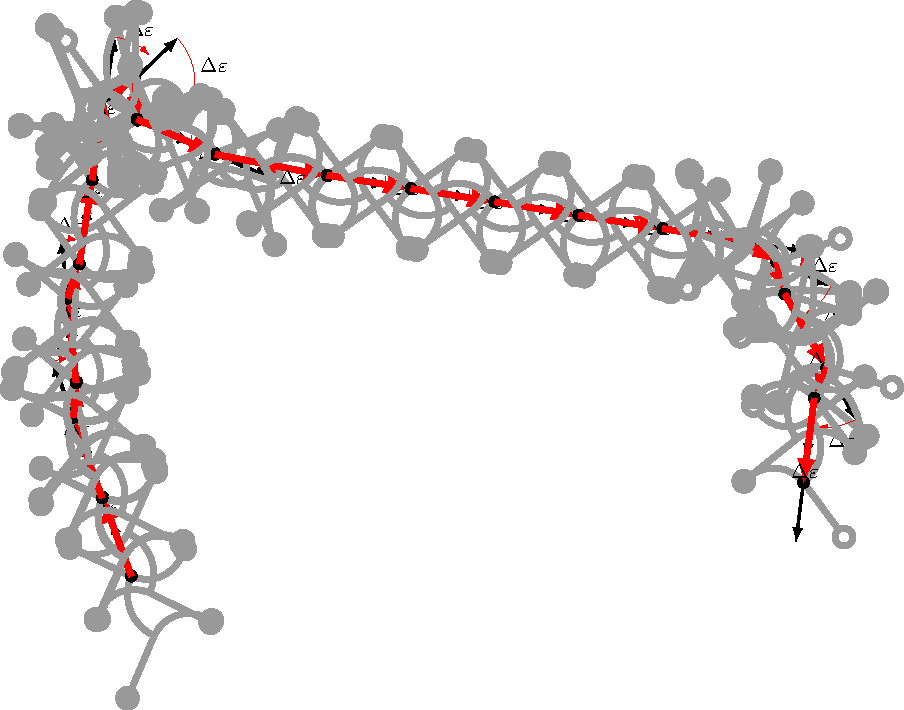
\includegraphics[scale=.4]{example2_.pdf}};


\path (9,4)node[below right, red, align=left]{
	{[straight]}*2 \\
	{[curve right, straight]}*2 \\
	{[straight]} \\
	{[curve right tight]} \\
	{[curve right super tight]} \\
	{[straight]} \\
	{[curve left]} \\
	{[straight]}*5 \\
	{[curve right]} \\
	{[curve right tight]} \\
	{[straight]} \\
	{[curve right tight]} \\
	{[straight]}};


\end{tikzpicture}
\end{document}